\documentclass[%
	11pt,
	a4paper,
	utf8,
	%twocolumn
		]{article}	

\usepackage{style_packages/podvoyskiy_article_extended}


\begin{document}
\title{Машинное обучение и анализ данных. Заметки}

\author{\itshape Подвойский А.О.}

\date{}
\maketitle

\thispagestyle{fancy}

Здесь приводятся заметки по некоторым вопросам, касающимся машинного обучения, анализа данных, программирования на языках \texttt{Python}, \texttt{R} и прочим сопряженным вопросам так или иначе, затрагивающим работу с данными.

\tableofcontents

\section{Градиентный бустинг}

\subsection{Общие сведения}

\subsection{Особенности реализации в \texttt{sklearn}}

\subsection{Особенности реализации в \texttt{XGBoost}}

\subsubsection{Установка пакета \texttt{xgboost} на \texttt{Windows}}

Устанавливать пакет \texttt{xgboost} рекомендуется с помощью следующей команды

\begin{lstlisting}[
numbers = none
]
conda install -c anaconda py-xgboost 
\end{lstlisting}

Существует альтернативный способ установки пакета \texttt{xgboost} (разумеется он работает и для других пакетов). Для начала требуется вывести список доступных каналов (см. \pic{fig:xgboost_conda_search}), по которым будет проводиться поиск интересующего пакета (в данном случае пакета \texttt{xgboost}), а затем можно воспользоваться конструкцией

\begin{lstlisting}[
numbers = none
]
anaconda search -t conda xgboost
\end{lstlisting}

\begin{figure}[h]
	\centering
	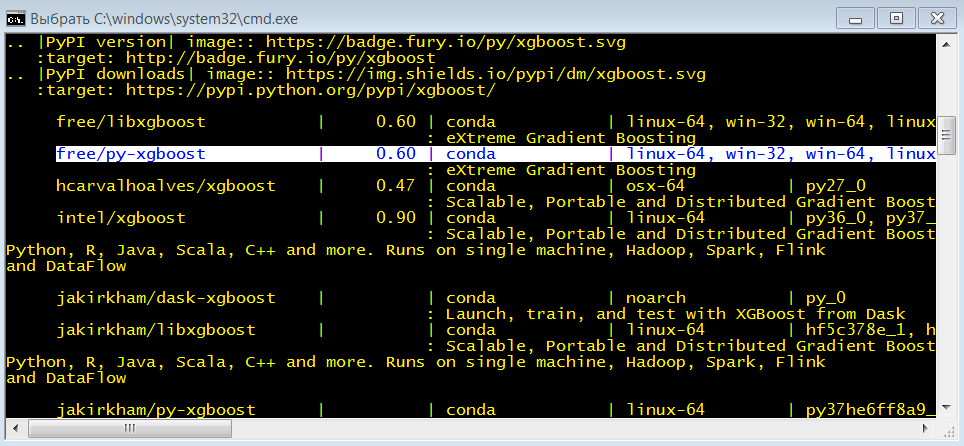
\includegraphics[scale=0.85]{figures/xgboost_conda_search.png}
	\caption{Окно командной оболочки \texttt{cmd.exe} со списком доступных каналов, по которым будет проводиться поиск пакета \texttt{xgboost} }\label{fig:xgboost_conda_search}
\end{figure}


После, выбрав канал, можно приступать к установке пакета

\begin{lstlisting}[
numbers = none
]
conda install -c free py-xgboost
\end{lstlisting}

\subsection{Простой пример работы с \texttt{xgboost} и \texttt{shap}}

Решается задача бинарной классификации. Требуется построить модель, предсказывающую годовой доход заявителя по порогу \$50'000 (то есть больше или меньше \$50'000 зарабатывает заявитель в год). Используется набор данных  UCI Adult income

\begin{lstlisting}[
style = ironpython,
numbers = none
]
import xgboost
import shap  # для оценки важности признаков вычисляются значения Шепли (Shapley value)
import numpy as np
import matplotlib.pyplot as plt
from sklearn.model_selection import train_test_split

shap.initjs()

X, y = shap.datasets.adult()
X_display, y_display = shap.datasets.adult(display=True)

X_train, X_test, y_train, y_test = train_test_split(X, y, test_size=0.2, random_state=7)
d_train = xgboost.DMatrix(X_train, label=y_train)
d_test = xgboost.DMatrix(X_test, label=y_test)

params = {
    'eta' : 0.01,
    'objective' : 'binary:logistic',
    'subsample' : 0.5,
    'base_score' : np.mean(y_train),
    'eval_metric' : 'logloss'        
}
model = xgboost.train(params, d_train,
                      num_boost_round = 5000,  # число итераций бустинга
                      evals = [(d_test, 'test')],
                      verbose_eval=100,  # выводит результат на каждой 100-ой итерации бустинга
                      early_stopping_rounds=20)

xgboost.plot_importance(model)
\end{lstlisting}

На \pic{fig:xgboost_plot}, \pic{fig:xgboost_plot_cover} и \pic{fig:xgboost_plot_gain} изображены графики важности признаков.

\begin{figure}[h]
	\centering
	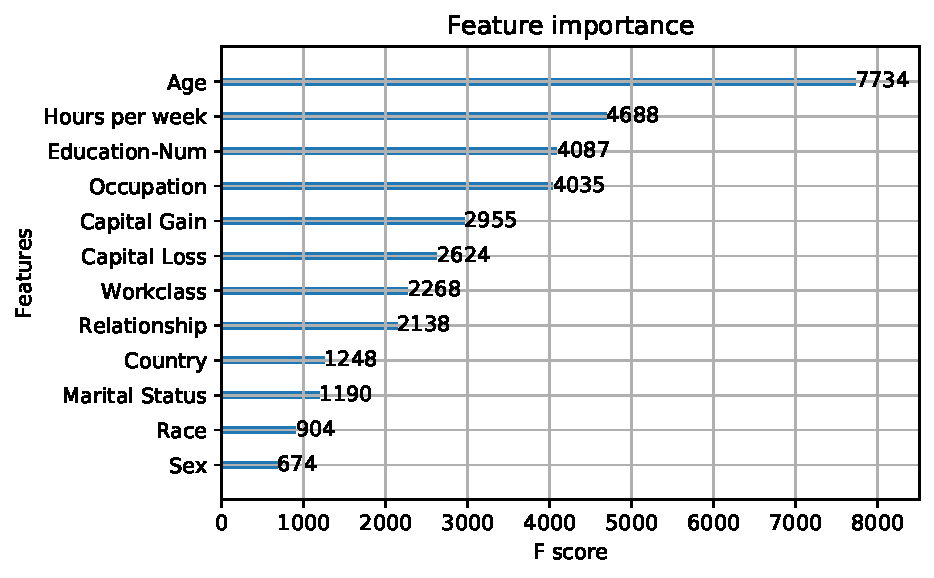
\includegraphics[scale=0.75]{figures/xgboost.plot.pdf}
	\caption{График важности признаков \lstinline{xgboost.plot_importance(model)},\\построенный с помощью пакета \texttt{xgboost} }\label{fig:xgboost_plot}
\end{figure}

\begin{figure}[h]
	\centering
	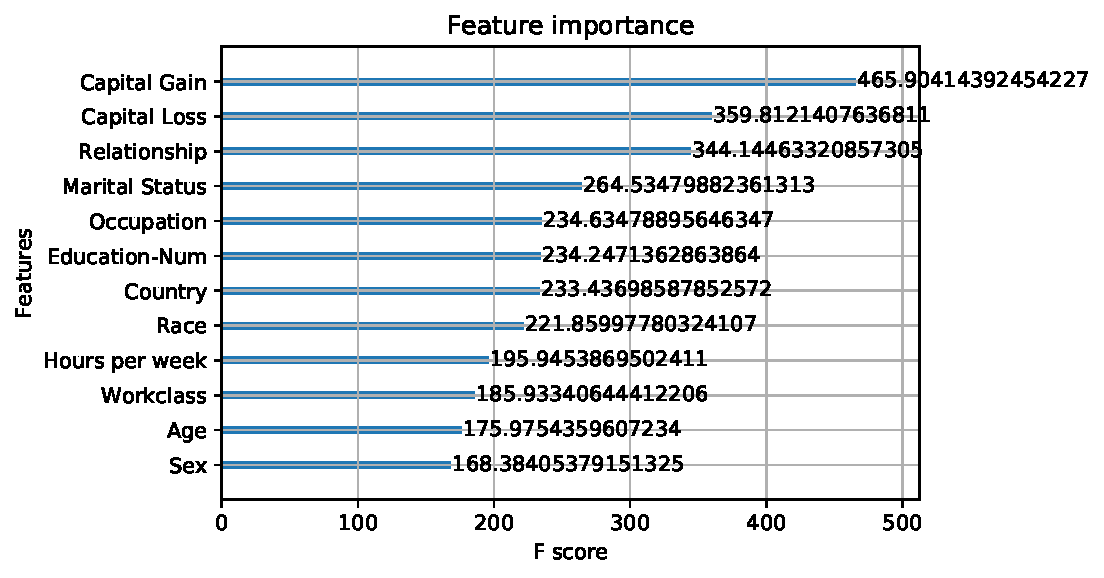
\includegraphics[scale=0.75]{figures/xgboost.plot.cover.pdf}
	\caption{График важности признаков \lstinline{xgboost.plot_importance(model, importance_type='cover')},\\построенный с помощью пакета \texttt{xgboost} }\label{fig:xgboost_plot_cover}
\end{figure}

\begin{figure}[h]
	\centering
	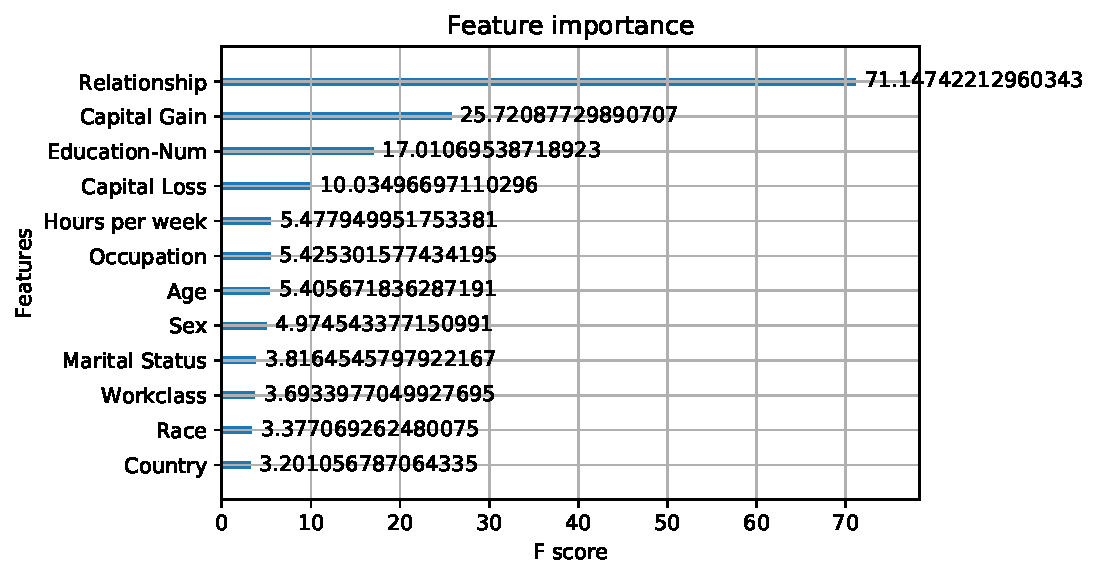
\includegraphics[scale=0.75]{figures/xgboost.plot.gain.pdf}
	\caption{График важности признаков \lstinline{xgboost.plot_importance(model, importance_type='gain')},\\построенный с помощью пакета \texttt{xgboost} }\label{fig:xgboost_plot_gain}
\end{figure}

Следует иметь в виду, что в библиотеке \texttt{xgboost} поддерживается три варианта вычисления важности признаков (см.~\href{https://towardsdatascience.com/interpretable-machine-learning-with-xgboost-9ec80d148d27}{Interpretable Machine Learning with XGBoost}):

\begin{itemize}
	\item \texttt{weight}: общее число сценариев по всем деревьям, когда $i$-ый признак используется для расщепления обучающего набора данных,
	
	\item \texttt{cover}: общее число сценариев по всем деревьям, когда $i$-ый признак используется для расщепления набора данных, взвешенное по числу точек обучающего набора данных, которые проходят через эти расщепления,
	
	\item \texttt{gain}: среднее снижение потерь на обучающем наборе данных, полученное при использовании $i$-ого признака.
\end{itemize}


\subsection{Особенности реализации в \texttt{LightGBM}}

\subsection{Особенности реализации в \texttt{CatBoost}}

\section{Приемы интерпретации моделей машинного обучения}

\section{Области видимости в языке \texttt{Python}}

Когда мы говорим о поиске значения имени применительно к программному коду, под термином \emph{область видимости} подразумевается \emph{пространство имен} -- то есть место в программном коде, где имени было присвоено значение \cite{lutz:learningpython-2011}.

В любом случае область видимости переменной (где она может использоваться) всегда определяется местом, где ей было присвоено значение.

\remark{%
Термины <<\emph{область видимости}>> и <<\emph{пространство имен}>> можно использовать как синонимичные
}

При каждом вызове функции создается новое \emph{локальное пространство имен}. Это пространство имен представляет локальное окружение, содержащее имена параметров функции, а также имена переменных, которым были присвоены значения в теле функции.

По умолчанию операция присваивания создает локальные имена (это поведение можно изменить с помощью \texttt{global} или \texttt{local}).

Схема разрешения имен в языке \texttt{Python} иногда называется \emph{правилом LEGB}\footnote{Local, Enclosing, Global, Built-in} \cite[\strbook{477}]{lutz:learningpython-2011}:

\begin{itemize}
	\item Когда внутри функции выполняется обращение к неизвестному имени, интерпретатор пытается отыскать его в четырех областях видимости -- в \emph{локальной}, затем в \emph{локальной области любой объемлющей функции} или в выражении \texttt{lambda}, затем в \emph{глобальной} и, наконец, во \emph{встроенной}. Поиск завершается, как только будет найдено первое подходящее имя.
	
	\item Когда внутри функции выполняется операция присваивания \lstinline{a=10} (а не обращения к имени внутри выражения), интерпретатор всегда создает или изменяет имя в \emph{локальной области видимости}, если в этой функции оно не было объявлено глобальным или нелокальным.
\end{itemize}

Пример

\begin{lstlisting}[
style = ironpython,
numbers = none
]
# глобальная область видимости
X = 99  

def func(Y):  # Y и Z локальные переменные
    # локальная область видимости
    Z = X + Y # X - глобальная переменная
    return Z
    
func(1)  # Y = 1
\end{lstlisting}

Переменные \texttt{Y} и \texttt{Z} являются \emph{локальными} (и существуют только во время выполнения функции), потому что присваивание значений обоим именам осуществляется внутри определения функции: присваивание переменной \texttt{Z} производится с помощью инструкции \texttt{=}, а \texttt{Y} -- потому что аргументы всегда передаются через операцию присваивания.

Когда внутри функции выполняется операция присваивания значения переменной, она всегда выполняется в \emph{локальном пространстве имен функции}

\begin{lstlisting}[
style = ironpython,
emph = {f},
numbers = none
]
a = 10  # глобальная область видимости

def f():
    a = 100  # локальная область видимости
    return a
\end{lstlisting}

В результате переменная \texttt{a} в теле функции ссылается на совершенно другой объект, содержащий значение 100, а не тот, на который ссылается внешняя переменная.

Переменные во вложенных функциях привязаны к \emph{лексической области видимости}. То есть поиск имени переменной начинается в \emph{локальной области видимости} и затем последовательно продолжается во всех \emph{объемлющих областях видимости внешних функций}, в направлении от внутренних к внешним.

Если и в этих \emph{пространствах имен} искомое имя не будет найдено, поиск будет продолжен в \emph{глобальном пространстве имен}, а затем во \emph{встроенном пространстве имен}, как и прежде.

При обращении к локальной переменной до того, как ей будет присвоено значение, возбуждается исключение \texttt{UnboundLocalError}. Следующий пример демонстрирует один из возможных сценариев, когда такое исключение может возникнуть

\begin{lstlisting}[
style = ironpython,
emph = {foo},
numbers = none
]
i = 0
def foo():
    i = i + 1  # приведет к исключению UnboundLocalError
    print(i)
\end{lstlisting}

В этой функции переменная \texttt{i} определяется как \emph{локальная} (потому что внутри функции ей присваивается некоторое значение и отсутствует инструкция \texttt{global}).

При этом инструкция присваивания \lstinline{i = i + 1} пытается прочитать значение переменной \texttt{i} еще до того, как ей будет присвоено значение.

Хотя в этом примере существует глобальная переменная \texttt{i}, она не используется для получения значения. Переменные в функциях могут быть либо \emph{локальными}, либо \emph{глобальными} и не могут произвольно изменять \emph{область видимости} в середине функции.

Например, нельзя считать, что переменная \texttt{i} в выражении \lstinline{i + 1} в предыдущем фрагменте обращается к глобальной переменной \texttt{i}; при этом переменная \texttt{i} в вызове \texttt{print(i)} подразумевает локальную переменную \texttt{i}, созданную в предыдущей инструкции.

\quinta{%
	Когда интерпретатор, сканируя определение функции \texttt{def}, натыкается на строку \texttt{i = i + 1}, он заключает что переменная \texttt{i} является \emph{локальной}, так как ей присваивается какое-то значение в теле функции. А когда функция вызывается на выполнение и интерпретатор снова доходит до строки \texttt{i = i + 1} выясняется, что переменная \texttt{i}, стоящая в правой части, не имет ссылок на какой-либо объект и потому возбуждается исключение \texttt{UnboundLocalError}
}

\section{Замыкания/фабричные функции в \texttt{Python}}

Под термином \emph{замыкание} или \emph{фабричная функция} подразумевается объект функции, который сохраняет значения в \emph{объемлющих областях видимости}, даже когда эти области могут прекратить свое существование \cite[\strbook{488}]{lutz:learningpython-2011}.

Замыкания и вложенные функции особенно удобны, когда требуется реализовать концепцию отложенных вычислений \cite{beazley:python-2010}.

Рассмотрим в качестве примера следующую функцию

\begin{lstlisting}[
title = {\sffamily Пример замыкания},
style = ironpython,
emph = {maker, action},
numbers = none
]
def maker(N):
    def action(X):
        return X**N  # функция action запоминает значение N в объемлющей области видимости
    return action
\end{lstlisting}

Здесь определяется внешняя функция, которая просто создает и возвращает вложенную функцию, не вызывая ее. Если вызвать внешнюю функцию

\begin{lstlisting}[
style = ironpython,
emph = {maker},
numbers = none
]
>>> f = maker(2)  # запишет 2 в N
>>> f  # <function action at 0x0147280>
\end{lstlisting}
она вернет ссылку на созданную ею вложенную функцию, созданную при выполнении вложенной инструкции \texttt{def}. Если теперь вызвать то, что было получено от внешней функции

\begin{lstlisting}[
style = ironpython,
numbers = none
]
>>> f(3)  # запишет 3 в X, в N по-прежнему хранится число 2
>>> f(4)  # 4**2
\end{lstlisting}
будет вызвана вложенная функция, с именем \texttt{action} внутри функции \texttt{maker}. Самое необычное здесь то, что вложенная функция продолжает хранить число 2, значение переменной \texttt{N} в функции \texttt{maker} даже при том, что к моменту вызова функции \texttt{action} функция \texttt{maker} уже \emph{завершила свою работу и вернула управление}.

Когда функция используется как вложенная, в замыкание включается все ее окружение, необходимое для работы внутренней функции \cite[\strbook{137}]{beazley:python-2010}.

\subsection{Области видимости и значения по умолчанию применительно к переменным цикла}

Существует одна известная особенность для функций или lambda-выражений: если lambda-выражение или инструкция \texttt{def} вложены в цикл внутри другой функции и вложенная функция ссылается на переменную из объемлющей области видимости, которая изменяется в цикле, все функции, созданные в этом цикле, будут иметь одно и то же значение -- значение, которое имела переменная на последней итерации \cite[\strbook{492}]{lutz:learningpython-2011}.

Например, ниже предпринята попытка создать список функций, каждая из которых запоминает текущее значение переменной \texttt{i} из объемлющей области видимости

\begin{lstlisting}[
title = {\sffamily Эта реализация работать НЕ будет},
style = ironpython,
emph = {makeActions},
numbers = none
]
def makeActions():
    acts = []
    for i in range(5):  # область видимости объемлющей функции
        acts.append(
            lambda x: i**x  # локальная область видимости вложенной анонимной функции
        ) 
    return acts
    
acts = makeActions()
print(acts[0](2))  # вернет 4**2, последнее значение i
print(acts[3](2))  # вернет 4**2, последнее значение i
\end{lstlisting}

Такой подход не дает желаемого результата, потому что поиск переменной в объемлющей области видимости производится позднее, \emph{при вызове вложенных функций}, в результате все они получат одно и то же значение (значение, которое имела переменная цикла на последней итерации).

Это один из случаев, когда необходимо явно сохранять значение из объемлющей области видимости в виде аргумента со значением по умолчанию вместо использования ссылки на переменную из объемлющей области видимости.

То есть, чтобы фрагмент заработал, необходимо передать текущее значение переменной из объемлющей области видимости в виде значения по умолчанию. Значения по умолчанию вычисляются в момент \emph{создания вложенной функции} (а не когда она \emph{вызывается}), поэтому каждая из них сохранит свое собственное значение \texttt{i}

\begin{lstlisting}[
title = {\sffamily Правильная реализация},
style = ironpython,
emph = {makeActions},
numbers = none
]
def makeActions():
    acts = []
    for i in range(5):
        acts.append(
            lambda x, i=i: i**x  # сохранить текущее значение i
        )
    return acts

acts = makeActions()
print(acts[0](2))  # вернет 0**2
print(acts[2](2))  # вернет 2**2
\end{lstlisting}

\quinta{%
Значения аргументов по умолчанию вложенных функций, динамически создаваемых в цикле на уровне области видимости объемлющей функции, вычисляются в момент \emph{создания} этих вложенных функций, а не в момент их вызова, поэтому \texttt{lambda x, i=i: ...} работает корректно
}


\section{Калибровка классификаторов}

Подробности в статье А. Дьяконова \href{https://dyakonov.org/2020/03/27/%D0%BF%D1%80%D0%BE%D0%B1%D0%BB%D0%B5%D0%BC%D0%B0-%D0%BA%D0%B0%D0%BB%D0%B8%D0%B1%D1%80%D0%BE%D0%B2%D0%BA%D0%B8-%D1%83%D0%B2%D0%B5%D1%80%D0%B5%D0%BD%D0%BD%D0%BE%D1%81%D1%82%D0%B8/}{<<Проблема калибровки уверенности>>}.
\vspace{2mm}

Ниже описываются способы оценить качество калибровки алгоритма. Надо сравнить \emph{уверенность} (confidence) и \emph{долю верных ответов} (accuracy) на тестовой выборке.

Если классификатор <<хорошо откалиброван>> и для большой группы объектов этот классификатор возвращает вероятность принадлежности к положительному классу 0.8, то среди этих объектов будет приблизительно 80\% объектов, которые в действительности принадлежат положительному классу. То есть, если для группы точек данных общим числом 100 классификатор возвращает вероятность положительного класса 0.8, то приблизительно 80 точек на самом деле будут принадлежать положительному классу и доля верных ответов тогда составит 0.8.

\subsection{Непараметрический метод гистограммной калибровки (Histogram Binning)}

Изначально в методе использовались бины одинаковой ширины, но можно использовать и равномощные бины.

Недостатки подхода:

\begin{itemize}
	\item число бинов задается наперед,
	
	\item функция деформации не непрерывна,
	
	\item в <<равноширинном варианте>> в некоторых бинах может содержаться недостаточное число точек.
\end{itemize}

Метод был предложен Zadrozny В. и Elkan C. \href{http://cseweb.ucsd.edu/~elkan/calibrated.pdf}{\ttfamily Obtaining  calibrated  probability  estimates  from  decision  trees  and naive bayesian classifiers}.

\subsection{Непараметрический метод изотонической регрессии (Isotonic Regression)}

Строится монотонно неубывающая функция деформации оценок алгоритма.

Метод был предложен Zadrozny B. и Elkan C. \href{http://citeseerx.ist.psu.edu/viewdoc/download?doi=10.1.1.13.7457&rep=rep1&type=pdf}{\ttfamily Transforming classifier scores into accurate multiclass probability estimates}.

Функция деформации по-прежнему не является непрерывной.

\subsection{Параметрическая калибровка Платта (Platt calibration)}

Изначально этот метод калибровки разрабатывался только для метода опорных векторов, оценки которого лежат на вещественной оси (по сути, это расстояния до оптимальной разделяющей классы прямой, взятые с нужным знаком). Считается, что этот метод не очень подходит для других моделей.

Предложен Platt~J. \href{http://citeseerx.ist.psu.edu/viewdoc/download;jsessionid=EA4888FEE74FB677B492740F59CDFE1F?doi=10.1.1.41.1639&rep=rep1&type=pdf}{\ttfamily Probabilistic  outputs  for  support  vector machines and comparisons to regularized likelihood methods}.

\subsection{Логистическая регрессия в пространстве логитов}

\subsection{Деревья калибровки}

Стандартный алгоритм строит строит суперпозицию дерева решений на исходных признаках и логистических регрессий (каждая в своем листе) над оценками алгоритма:

\begin{itemize}
	\item Построить на исходных признаках решающее дерево (не очень глубокое),
	
	\item В каждом листе -- обучить логистическую регрессию на одном признаке,
	
	\item Подрезать дерево, минимизируя ошибку.
\end{itemize}

\subsection{Температурное шкалирование (Temperature Scaling)}

Этот метод относится к классу DL-методов калибровки, так как он был разработан именно для калибровки нейронных сетей. Метод представляет собой простое многомерное обобщение шкалирования Платта.

\section{Приемы работы с менеджером пакетов \texttt{conda}}

\subsection{Создание виртуального окружения}

Создать виртуальное окружение \texttt{dashenv}

\begin{lstlisting}[
numbers = none
]
conda create --name dashenv
\end{lstlisting}

Создать виртуальное окружение с указанием версии \texttt{Python}

\begin{lstlisting}[
numbers = none
]
conda create --name testenv python=3.6
\end{lstlisting}

Создать виртуальное окружение с указанием пакета

\begin{lstlisting}[
numbers = none
]
conda create --name testenv scipy
\end{lstlisting}

Создать виртуальное окружение с указанием версии \texttt{Python} и нескольких пакетов

\begin{lstlisting}[
numbers = none
]
conda create --name testenv python=3.6 scipy=0.15.0 astroid babel
\end{lstlisting}

\remark{%
Рекомендуется устанавливать сразу несколько пакетов, чтобы избежать конфликта зависимостей
}

Для того чтобы при создании нового виртуального окружения не требовалось каждый раз устанавливать базовые пакеты, которые обычно используются в работе, можно привести их список в конфигурационном файле \texttt{.condarc} в разделе \texttt{create\_default\_packages}

\begin{lstlisting}[
title = {\sffamily .condarc},
numbers = none
]
ssl_verify: true
channels:
 - conda-forge
 - defaults
report_errors: true
default_python:
create_default_packages:
 - matplotlib
 - numpy
 - scipy
 - pandas
 - seaborn
\end{lstlisting}

Если для текущего виртуального окружения не требуется устанавливать пакеты из набора по умолчанию, то при создании виртуального окружения следует указать специальный флаг
\lstinline{--no-default-packages}

\begin{lstlisting}[
numbers = none
]
conda create --no-default-packages --name testenv python
\end{lstlisting}

Создать виртуальное окружение можно и из файла \texttt{environment.yml} (первая строка этого файла станет именем виртуального окружения)

\begin{lstlisting}[
title = {\sffamily environment.yml},
numbers = none
]
name: stats2
channels:
 - conda-forge
 - defaults
dependencies:
 - python=3.6   # or 2.7
 - bokeh=0.9.2
 - numpy=1.9.*
 - nodejs=0.10.*
 - flask
 - pip:
  - Flask-Testing
\end{lstlisting}

\begin{lstlisting}[
numbers = none
]
conda env create -f environment.yml
\end{lstlisting}

При создании виртуального окружения можно указать путь до целевой директории, где будут размещаться файлы окружения. Следующая команда создаст виртуальное окружение в поддиректории текущей рабочей директории \texttt{envs}\footnote{В данном случае чтобы удалить виртуальную среду достачно просто удалить директорию \texttt{envs}}

\begin{lstlisting}[
numbers = none
]
conda create --prefix ./envs jupyterlab matplotlib
\end{lstlisting}

С помощью файла спецификации можно создать \emph{идентичное виртуальное окружение} (i) на той же платформе операционной системы, (ii) на той же машине, (iii) на какой-либо другой машине (перенести настройки окружения).

Для этого предварительно требуется создать собственно файл спецификации

\begin{lstlisting}[
numbers = none
]
conda list --explicit > spec-file.txt
\end{lstlisting}

Имя файла спецификации может быть любым. Файл спецификации обычно не является кросс-платформенным и поэтому имеет комментарий в верхней части файла (\lstinline{#platform: osx-64}), указывающий платформу, на которой он был создан.

Теперь для того чтобы \emph{создать} окружение достаточно воспользоваться командой

\begin{lstlisting}[
numbers = none
]
conda create --name myenv --file spec-file.txt
\end{lstlisting}

Файл спецификации можно использовать для установки пакетов в существующее окружение

\begin{lstlisting}[
numbers = none
]
conda install --name myenv --file spec-file.txt
\end{lstlisting}


\subsection{Активация/деактивация виртуального окружения}

Активировать виртуальное окружение \texttt{dashenv}

\begin{lstlisting}[
numbers = none
]
conda activate dashenv
\end{lstlisting}

Активировать виртуальное окружение в случае, когда оно создавалось с \lstinline{--prefix}, можно указав полный путь до окружения
\begin{lstlisting}[
numbers = none
]
conda activate E:\[WorkDirectory]\[Python_projects]\directory_for_experiments\envs
\end{lstlisting}

В этом случае в строке приглашения командной оболочки по умолчанию будет отображаться полный путь до окружения. Чтобы заменить длинный префикс в имени окружения на более удобный псевдоним достаточно использовать конструкцию

\begin{lstlisting}[
numbers = none
]
conda config --set env_prompt ({name})
\end{lstlisting}
которая добавит в конфигурационный файл \texttt{.condarc} следующую строку

\begin{lstlisting}[
title = {\sffamily .condarc},
numbers = none
]
...
env_prompt: ({name})
\end{lstlisting}
и теперь имя окружения будет \texttt{(envs)}.

Деактивировать виртуальное окружение

\begin{lstlisting}[
numbers = none
]
conda deactivate
\end{lstlisting}

\subsection{Обновление виртуального окружения}

Обновить виртуальное окружение может потребоваться в следующих случаях:

\begin{itemize}
	\item обновилась одна из ключевых зависимостей,
	
	\item требуется добавить пакет (добавление зависимости),
	
	\item требуется добавить один пакет и удалить другой.
\end{itemize}

В любом из этих случаев все что нужно для того чтобы обновить виртуальное окружение это просто обновить файл \texttt{environment.yml}\footnote{Этот файл должен находится в той же директории что и директория окружения \texttt{envs}}, а затем запустить команду

\begin{lstlisting}[
numbers = none
]
conda env update --prefix ./envs --file environment.yml --prune
\end{lstlisting}

Опция \lstinline{--prune} приводит к тому, что \texttt{conda} удаляет все зависимости, которые больше не нужны для окружения.

\subsection{Вывод информации о виртуальном окружении}

Вывести список доступных виртуальных окружений

\begin{lstlisting}[
numbers = none
]
conda env list
\end{lstlisting}

Вывести список пакетов, установленных в указанном окружении

\begin{lstlisting}[
numbers = none
]
conda list --name myenv
\end{lstlisting}

Вывести информацию по конкретному пакету указанного окружения

\begin{lstlisting}[
numbers = none
]
conda list --name dashenv matplotlib
\end{lstlisting}


\subsection{Удаление виртуального окружения}

Удалить виртуальное окружение \texttt{heroku\_env}

\begin{lstlisting}[
numbers = none
]
conda env remove --name heroku_env
\end{lstlisting}

\subsection{Экспорт виртуального окружения в \texttt{environment.yml}}

Экспортировать активное виртуальное окружение в yml-файл

\begin{lstlisting}[
numbers = none
]
conda env export > environment.yml
\end{lstlisting}

\section{Приемы работы с пакетом \texttt{Vowpal Wabbit}}

\section{Приемы работы с библиотекой \texttt{pandas}}

\subsection{Число уникальных значений категориальных признаков в объекте \texttt{DataFrame}}

Для того чтобы вывести информацию по числу уникальных значений в каждом категориальном признаке некоторого объекта \texttt{pandas.DataFrame} можно воспользоваться конструкцией

\begin{lstlisting}[
style = ironpython,
numbers = none
]
X.select_dtypes('category').apply(lambda col: col.unique().shape[0])
\end{lstlisting}

\subsection{Число пропущенных значений в объекте \texttt{DataFrame}}

Информацию по числу пропущенных значений в каждом столбце можно вывести следующим образом

\begin{lstlisting}[
style = ironpython,
numbers = none
]
X.isna().any(axis=0)
\end{lstlisting}


\section{Интерпретация моделей и оценка важности признаков с библиотекой \texttt{SHAP}}

\subsection{Общие сведения о значениях Шепли}

В библиотеке \texttt{SHAP} \url{https://github.com/slundberg/shap} для оценки \emph{важности признаков} используются \emph{значения Шепли} (Shapley value) \url{https://en.wikipedia.org/wiki/Shapley_value}.

Формула для вычисления значения Шепли $i$-ого признака имеет вид (здесь сумма распространяется на все подмножества $ S $ из множества признаков $ N $, не содержащие $ i $-ого признака)
\begin{align*}
\phi_i(v) = \sum_{S \subseteq N\setminus\{i\}} \dfrac{|S|!(n - |S| - 1)!}{n!}\Bigl( v(S \cup \{i\}) - v(S) \Bigr),
\end{align*}
где $ n $ -- общее число признаков; $ v(S \cup \{i\}) $ -- прогноз модели с учетом $ i $-ого признака; $ v(S) $ -- прогноз модели без $ i $-ого признака; $ S $ -- произвольный набор признаков без $ i $-ого признака.

Значение Шепли для $ i $-ого признака вычисляется для каждой точки данных (например, для каждого клиента в выборке) на всех возможных комбинациях признаков (в том числе и для пустых множеств $ S $). Затем полученные оценки суммируются по модулю, что в итоге дает важность $ i $-ого признака.

Библиотека \texttt{SHAP} позволяет интерпретировать и модель в целом, и результаты отдельных примеров \url{https://habr.com/ru/company/homecredit/blog/479712/}.


\subsection{Перестановочная важность признаков в библиотеке \texttt{eli5}}


Еще важность признаков можно оценивать с помощью так называемой \emph{перестановочной важности} (permutation importances) \url{https://www.kaggle.com/dansbecker/permutation-importance}.

Идея проста: нужно в заранее отведенном для исследования важности признаков наборе данных (валидационном наборе) перетасовать значения признака, влияние которого изучается на данной итерации, оставив остальные признаки (столбцы) и целевой вектор без изменения.

Признак считается <<важным>>, если метрики качества модели падают, и соответственно -- <<неважным>>, если перестановка не влияет на значения метрик.

\remark{
Перестановочная важность вычисляется после того как модель будет обучена
}

Рассмотрим задачу построения регрессионной модели на наборе данных \texttt{load\_boston}

\begin{lstlisting}[
style = ironpython,
numbers = none
]
import eli5
import pandas as pd
from eli5.sklearn import PermutationImportance
from sklearn.ensemble import RandomForestRegressor
from sklearn.model_selection import train_test_split
from sklearn.datasets import load_boston
from pandas import DataFrame, Series

boston = load_boston()

X_train, X_test, y_train, y_test = train_test_split(boston['data'],
                                                    boston['target'], 
                                                    random_state=2)

X_train_sub, X_valid, y_train_sub, y_valid = train_test_split(X_train,
                                                              y_train,
                                                              random_state=0)

# модель случайного леса, как обычно, обучается на обучающей выборке
rf = RandomForestRegressor(n_estimators=500).fit(X_train_sub, y_train_sub)

# модель перестановочной важности обучается на валидационном наборе данных
perm = PermutationImportance(rf, random_state=42).fit(X_valid, y_valid)

eli5.show_weights(perm, feature_names = boston['feature_names'])  # визуализирует перестановочные важности признаков
\end{lstlisting}



% Источники в "Газовой промышленности" нумеруются по мере упоминания 
\begin{thebibliography}{99}\addcontentsline{toc}{section}{Список литературы}
	\bibitem{lutz:learningpython-2011}{{\emph{Лутц М.} Изучаем Python, 4-е издание. -- Пер. с англ. -- СПб.: Символ-Плюс, 2011. -- 1280~с. }
		
	\bibitem{beazley:python-2010}{\emph{Бизли Д.} Python. Подробный справочник. -- Пер. с англ. -- СПб.: Символ-Плюс, 2010. -- 864~с. }
	
	\bibitem{chacon:2020}{ \emph{Чакон С.}, \emph{Штрауб Б.} Git для профессионального программиста. -- СПб.: Питер, 2020. -- 496~с. }
	
\end{thebibliography}

%\listoffigures\addcontentsline{toc}{section}{Список иллюстраций}

\end{document}
